% !TeX root = ../../../main.tex
\subsection{Experiments}

We benchmark \ChTwoSmallCaps{Temporal-SCL} on tabular time series data:
a synthetic dataset with known ground truth embedding space structure (Section~\ref{ch02:sec:ToyExperiment}), and two standard real clinical datasets with unknown embedding space structure (Section~\ref{ch02:sec:ClinicalExperiments}). %
We also examine how \ChTwoSmallCaps{Temporal-SCL} works without pre-training and, separately, without nearest neighbor pairing.

As baselines, we use (a) purely supervised methods: logistic regression, an LSTM~\citep{hochreiter1997long}, \mbox{RETAIN} \citep{choi2016retain}, Dipole \citep{ma2017dipole}, a BERT-based transformer \citep{devlin2018bert}; (b) temporal predictive clustering methods: AC-TPC \citep{lee2020temporal} and T-Phenotype \citep{qin2023t}; and (c) Self-Supervised Learning and Contrastive Learning based model: SMD-SSL \citep{raghu2023sequential} with SimCLR loss \citep{chen2020simple} and VICReg loss \citep{bardes2021vicreg}, and \mbox{\ChTwoSmallCaps{Simple-SCL}} (treating snapshots as separate data points and without nearest neighbor pairing).
Details on baselines are in Appendix~\ref{ch02:sec:baselines}.

For all datasets, we randomly split the data into 60\% training, 20\% validation, and 20\% test sets. 
This split is done at the patient level so the presented test set results are all on patients not encountered during training.
Details of our training including network types and hyperparameter grids, and an explanation of evaluation metrics are in Appendix~\ref{ch02:sec:ExperimentalSetup}.
\footnote{Our code is available at: \\ \url{https://github.com/Shahriarnz14/Temporal-Supervised-Contrastive-Learning}}

   
\subsubsection{Synthetic Data}



% !TeX root = ../../../main.tex
\begin{figure}[!t]
\ChTwoFloatContents
    {ch02:fig:toyDataset}%
    {\caption{Synthetic dataset: panel (a) shows the only 4 possible time series trajectories (each true embedding vector state has a unique color-shape combination; there are 10 such states); every time series has 3 time steps and belongs to one of two classes \textcolor{red}{red}/\textcolor{blue}{blue}. Panels (b)-(e) show learned embedding spaces of four methods; only \ChTwoSmallCaps{Temporal-SCL} correctly recovers the 10 ground truth states. A version of this figure with embeddings of all methods evaluated is in Fig.~\ref{ch02:fig:toyDataset_result_complete}.
    }}%
    {%
     
        \subfigure[Ground truth]{%
            \label{ch02:fig:toyDataset_Raw}
            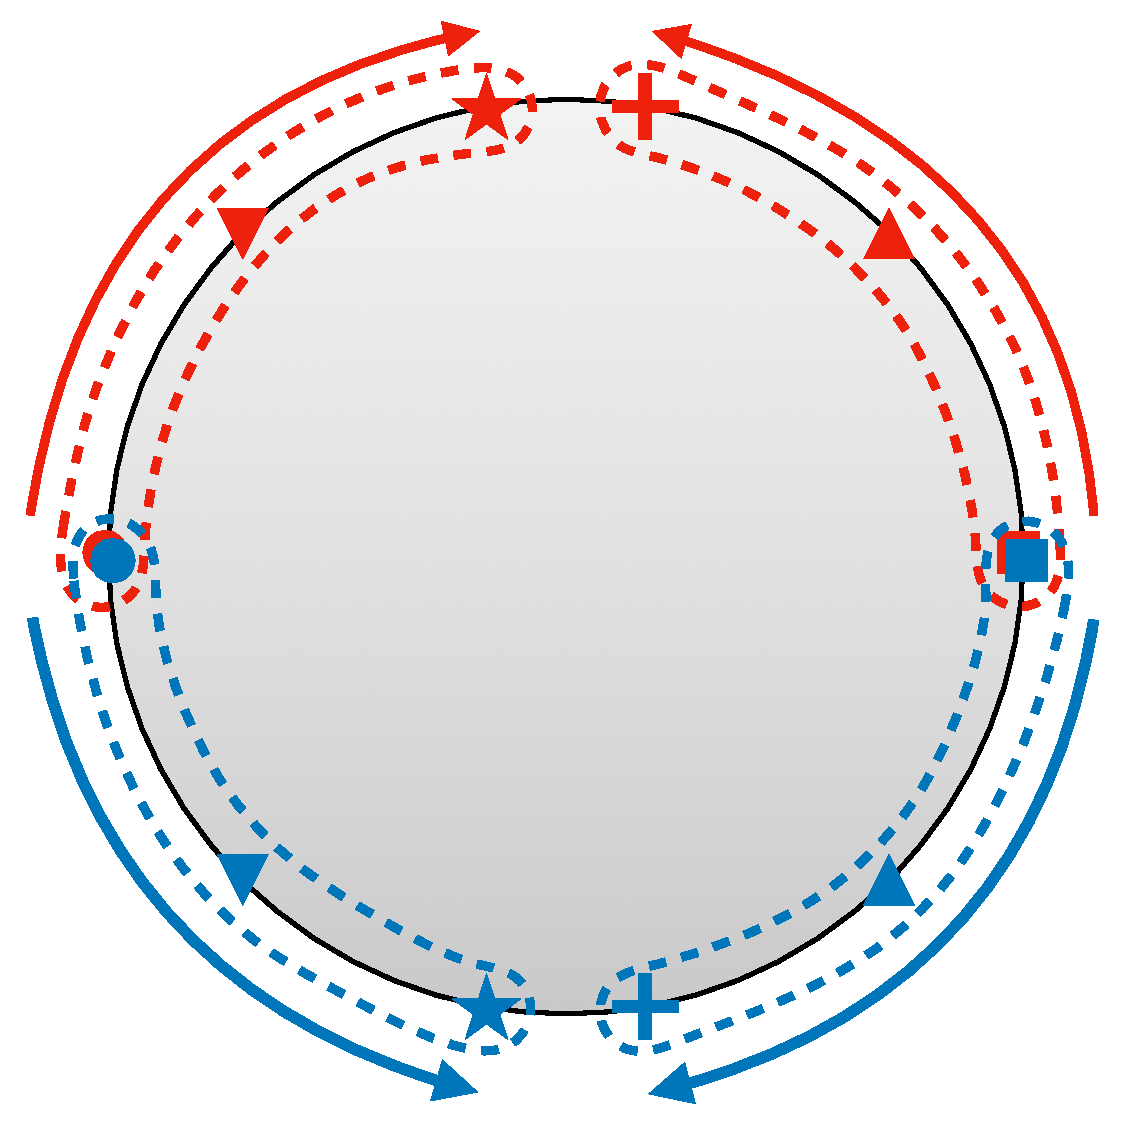
\includegraphics[width=0.195\linewidth]{Chapters/chapter-02/images/synthetic.pdf}
        }
        \subfigure[Transformer]{%
            \label{ch02:fig:synth-transformer}%
            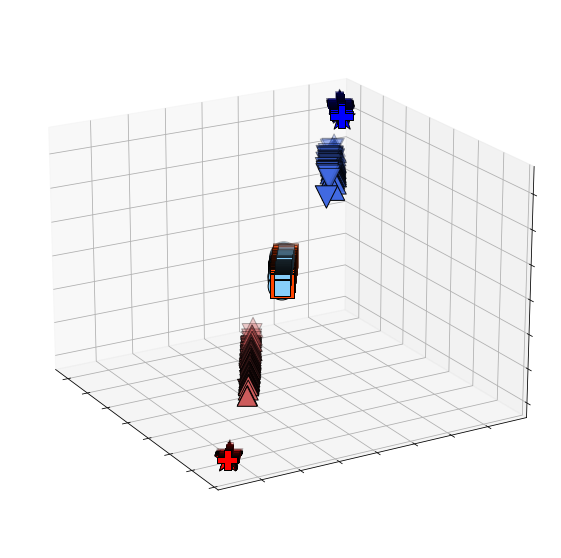
\includegraphics[width=0.18\linewidth]{Chapters/chapter-02/images/Embedding_Transformer.png}
        }
        \subfigure[T-Phenotype]{%
            \label{ch02:fig:synth-tphenotype}%
            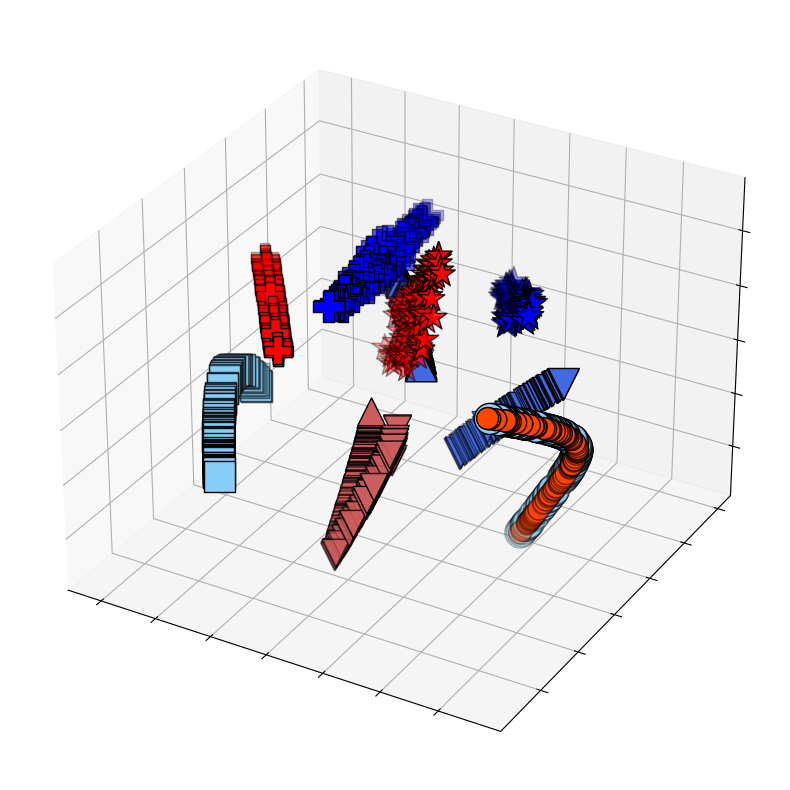
\includegraphics[width=0.18\linewidth]{Chapters/chapter-02/images/Embedding_TPhenotype.png}
        }
        \subfigure[\small\ChTwoSmallCaps{Temporal-SCL} \newline (no NN pairing)]{%
            \label{ch02:fig:synth-tscl-no-nnp}%
            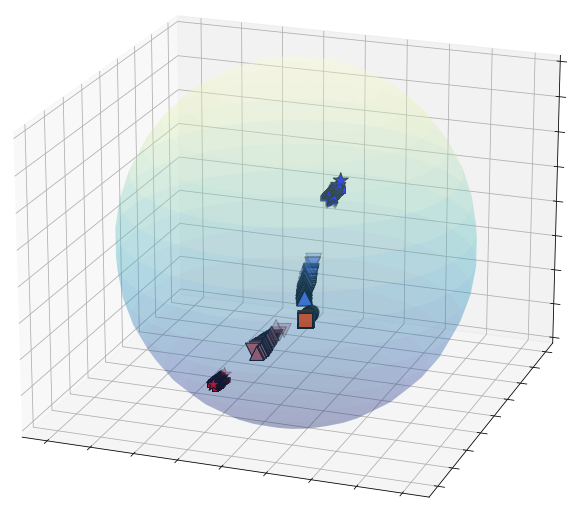
\includegraphics[width=0.18\linewidth]{Chapters/chapter-02/images/Embedding_NoKNN.png}
        }
        ~
        \subfigure[\small\ChTwoSmallCaps{Temporal-SCL}]{%
            \label{ch02:fig:synth-tscl}%
            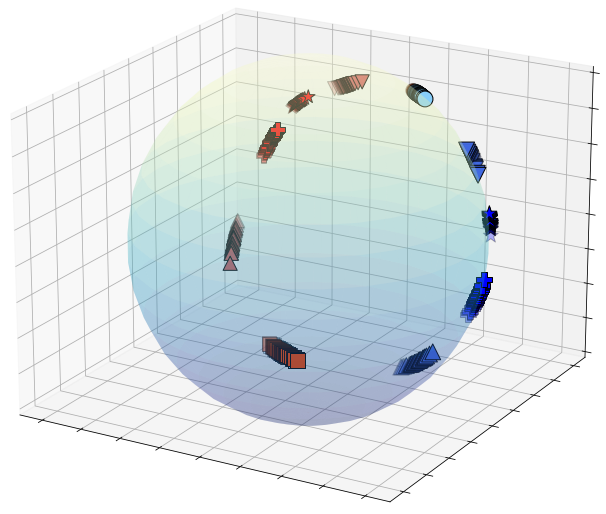
\includegraphics[width=0.18\linewidth]{Chapters/chapter-02/images/Embedding_TSCL.png}
        }
    }
\end{figure}

 
\label{ch02:sec:ToyExperiment}

\noindent
\textbf{Data.}
We generate a 2D dataset where every patient time series has exactly 3 time steps.
For simplicity, we only consider the static outcome case so that each time series has a single label (one of two classes: \textcolor{red}{red} or \textcolor{blue}{blue}).
The points are all on a 2D circle, where the only 4 possible time series in the embedding space are shown in Fig.~\ref{ch02:fig:toyDataset_Raw}. 
For example, one possible patient time series is ``\scalerel*{
\includegraphics{Chapters/chapter-02/images/circle-blue.pdf}}{B} $\rightarrow$ \scalerel*{
\includegraphics{Chapters/chapter-02/images/triangle-down-blue.pdf}}{B} $\rightarrow$ \scalerel*{
\includegraphics{Chapters/chapter-02/images/star-blue.pdf}}{B}''.
There are a total of 10 true embedding vector locations, which could be thought of as cluster centers. \emph{Note that we take the embedding space and raw feature space to be the same.} When we generate synthetic time series, each point is based on one of the 10 true ground truth embedding vector locations with Gaussian noise added.
We randomly sample 200 of each of the 4 possible trajectories so that we have a total of 800 time series.
See Appendix~\ref{ch02:sec:syntheticData_full} for details.


% !TeX root = ../../../main.tex
\begin{table}[t]

\caption{Synthetic data test set metrics %
(mean $\pm$ std.~dev.~across 10 experiments) and qualitative assessment of successful ground truth cluster recovery across experiments.}
\centering
\adjustbox{max width=.85\linewidth}{%
\begin{tabular}{cccccc}
\toprule
Model & AUROC & AUPRC & Silhouette Index & \shortstack[c]{Cluster Prediction\\ Accuracy} & Recovery \\ \midrule
Logistic Regression                         & 0.90$\pm$0.01 & 0.90$\pm$0.00 & 0.09$\pm$0.01 & 0.60$\pm$0.06 & \ChTwoXmark \\
LSTM                                        & 0.95$\pm$0.01 & 0.95$\pm$0.00 & 0.09$\pm$0.01 & 0.60$\pm$0.05 & \ChTwoXmark \\
RETAIN                                      & 0.95$\pm$0.01 & 0.95$\pm$0.00 & 0.33$\pm$0.06 & 0.69$\pm$0.06 & \ChTwoOmark \\
DIPOLE                                      & 0.95$\pm$0.01 & 0.95$\pm$0.00 & 0.30$\pm$0.06 & 0.69$\pm$0.04 & \ChTwoOmark \\
Transformer:BERT                            & 0.95$\pm$0.01 & 0.95$\pm$0.00 & 0.11$\pm$0.01 & 0.67$\pm$0.03 & \ChTwoXmark \\
AC-TPC                                      & 0.95$\pm$0.01 & 0.95$\pm$0.00 & 0.09$\pm$0.01 & 0.77$\pm$0.03 & \ChTwoXmark  \\
T-Phenotype                                 & 0.95$\pm$0.01 & 0.95$\pm$0.00 & 0.49$\pm$0.32 & 0.81$\pm$0.03 & \ChTwoOmark \\
SMD-SSL + SimCLR (Frozen)                   & 0.84$\pm$0.01 & 0.83$\pm$0.00 & 0.15$\pm$0.05 & 0.61$\pm$0.02 & \ChTwoOmark  \\
SMD-SSL + VICReg (Frozen)                   & 0.79$\pm$0.01 & 0.79$\pm$0.00 & 0.12$\pm$0.05 & 0.60$\pm$0.03 & \ChTwoOmark  \\
SMD-SSL + SimCLR (Fine-tune)                & 0.94$\pm$0.01 & 0.94$\pm$0.00 & 0.39$\pm$0.10 & 0.78$\pm$0.04 & \ChTwoOmark  \\
SMD-SSL + VICReg (Fine-tune)                & 0.95$\pm$0.01 & 0.95$\pm$0.00 & 0.24$\pm$0.12 & 0.73$\pm$0.04 & \ChTwoOmark  \\       
\cmidrule(lr){1-6}
\ChTwoSmallCaps{Simple-SCL} / \ChTwoSmallCaps{Temporal-SCL} (PT:\ChTwoXbmark, NN:\ChTwoXbmark, TR:\ChTwoXbmark)                                             & 0.93$\pm$0.01 & 0.94$\pm$0.01 & 0.19$\pm$0.01 & 0.64$\pm$0.06 & \ChTwoXmark \\
\ChTwoSmallCaps{Temporal-SCL} (PT:\ChTwoCbmark, NN:\ChTwoXbmark, TR:\ChTwoXbmark)      & 0.94$\pm$0.01 & 0.94$\pm$0.00 & 0.24$\pm$0.01 & 0.62$\pm$0.06 & \ChTwoXmark \\
\ChTwoSmallCaps{Temporal-SCL} (PT:\ChTwoXbmark, NN:\ChTwoCbmark, TR:\ChTwoXbmark)      & 0.94$\pm$0.01 & 0.95$\pm$0.00 & 0.82$\pm$0.01 & 0.84$\pm$0.05 & \ChTwoOmark \\
\ChTwoSmallCaps{Temporal-SCL} (PT:\ChTwoXbmark, NN:\ChTwoXbmark, TR:\ChTwoCbmark)      & 0.95$\pm$0.01 & 0.95$\pm$0.00 & 0.40$\pm$0.01 & 0.57$\pm$0.04 & \ChTwoXmark \\
\ChTwoSmallCaps{Temporal-SCL} (PT:\ChTwoXbmark, NN:\ChTwoCbmark, TR:\ChTwoCbmark)      & 0.95$\pm$0.01 & 0.94$\pm$0.00 & 0.86$\pm$0.00 & 0.91$\pm$0.06 & \ChTwoOmark \\
\ChTwoSmallCaps{Temporal-SCL} (PT:\ChTwoCbmark, NN:\ChTwoXbmark, TR:\ChTwoCbmark)      & 0.95$\pm$0.01 & 0.95$\pm$0.00 & 0.55$\pm$0.01 & 0.56$\pm$0.05 & \ChTwoXmark \\
\ChTwoSmallCaps{Temporal-SCL} (PT:\ChTwoCbmark, NN:\ChTwoCbmark, TR:\ChTwoXbmark)      & 0.95$\pm$0.01 & 0.95$\pm$0.00 & 0.92$\pm$0.01 & 0.85$\pm$0.03 & \ChTwoOmark \\
\ChTwoSmallCaps{Temporal-SCL} (Full)                                    & 0.95$\pm$0.01 & 0.95$\pm$0.00 & {\ChTwoBfTab 0.98$\pm$0.00} & {\ChTwoBfTab 1.00$\pm$0.00} & {\ChTwoBfTab \ChTwoCmark}   \\ 
\bottomrule
\end{tabular}}


{\scriptsize {\ChTwoBfTab{PT}}: Pre-Training, {\ChTwoBfTab{NN}}: Nearest Neighbor pairing, {\ChTwoBfTab{TR}}: Temporal Regularization}


{\scriptsize \ChTwoXmark: No correct recovery of the embedding structure.}


{\scriptsize \ChTwoOmark: Partial clustering structure found, but not a completely correct recovery of the embedding structure.}


{\scriptsize \ChTwoCmark: Completely correct recovery of the embedding structure.}
\ChTwoFloatLabel{ch02:tab:toyDataset_ratios}

\end{table}



\noindent
\textbf{Experimental results.}
We use a 3D embedding space for all methods despite the ground truth being~2D.\footnote{Confining the embedding space to 2D markedly degraded performance across all methods. We speculate that this due to ``over-specification'', aligned with findings in studies like \citet{livni2014computational} that suggest that training larger-than-necessary neural networks results in easier training.}
Fig.~\ref{ch02:fig:toyDataset} depicts the test data projected onto a 3D embedding space of a few different methods (in the appendix, Fig.~\ref{ch02:fig:toyDataset_result_complete} has visualizations across all methods evaluated). 
We report test set accuracy scores for predicting red/blue (area under the ROC curve, area under precision recall curve), silhouette index (SI) using ground truth cluster centers as cluster labels, and lastly a qualitative analysis of whether all 10 clusters were recovered across the 10 experimental repeats (this is a qualitative visual check) in Table~\ref{ch02:tab:toyDataset_ratios}. 
Additionally, we also investigate a different downstream task focusing on cluster prediction accuracy.
In this task, we freeze the encoder network, previously trained on the synthetic data, and task the model with predicting the cluster location for each timestep.
This experiment is used to evaluate the model's ability to be used for different downstream tasks and evaluate whether the trained encoder can correctly identify the cluster of origin for each data point within the synthetic dataset's defined 10 clusters (as shown in Fig.~\ref{ch02:fig:toyDataset_Raw}).
The cluster prediction accuracy is reported alongside other results in Table~\ref{ch02:tab:toyDataset_ratios}.

The main finding from our synthetic data experiment is that while most methods yield similar, optimal prediction scores, only the full version of \ChTwoSmallCaps{Temporal-SCL} consistently recovers all 10 clusters.
This is evident in the high silhouette index (0.98) our full model achieves, closely matching the ground truth SI of 0.982. %
This claim is further supported by visual examination of Fig.~\ref{ch02:fig:toyDataset} (also see the last column of Table~\ref{ch02:tab:toyDataset_ratios} and appendix Fig.~\ref{ch02:fig:toyDataset_result_complete}).
No other method evaluated consistently recovers all 10 ground truth clusters.
Notably, removing nearest neighbor pairing from \ChTwoSmallCaps{Temporal-SCL} leads to a 0\% recovery rate of ground truth clusters. 
Lastly, our full model is the only one among all baselines and ablations to achieve 100\% accuracy in the downstream task of cluster prediction.
This result highlights our model's ability to accurately identify cluster origins and provides empirical evidence of the versatility of the learned encoder representations for a different downstream task.


   
\subsubsection{Real Clinical Data}
\label{ch02:sec:ClinicalExperiments}



% !TeX root = ../../../main.tex
\begin{table}[t]
\caption{Real data test set accuracy (mean $\pm$ std.~dev.~across 10 experiments).}
\centering
\adjustbox{max width=.8\linewidth}{%
\begin{tabular}{ccccc} 
\toprule
                        \multirow{2}{*}[-2pt]{Model}           & \multicolumn{2}{c}{MIMIC dataset}                  & \multicolumn{2}{c}{ADNI dataset}                                                   
                                                                        \\ \cmidrule(lr){2-3} \cmidrule(lr){4-5} %
                                                               & AUROC                      & AUPRC                   & AUROC                   & AUPRC \\ 
                        \midrule
                        Logistic Regression                    & 0.745$\pm$0.003            & 0.499$\pm$0.008         & 0.845$\pm$0.006          & 0.676$\pm$0.009 \\
					  LSTM                                   & 0.767$\pm$0.003            & 0.509$\pm$0.005         & 0.947$\pm$0.002          & 0.823$\pm$0.005 \\
                        RETAIN                                 & 0.730$\pm$0.010            & 0.431$\pm$0.006         & 0.884$\pm$0.012          & 0.795$\pm$0.016 \\
                        DIPOLE                                 & 0.767$\pm$0.004            & 0.453$\pm$0.003         & 0.958$\pm$0.006          & 0.824$\pm$0.009 \\
                        Transformer:BERT                       & 0.769$\pm$0.005            & 0.509$\pm$0.003         & 0.959$\pm$0.002          & 0.922$\pm$0.003 \\                        
                        AC-TPC                                 & 0.703$\pm$0.006            & 0.432$\pm$0.007         & 0.839$\pm$0.013          & 0.681$\pm$0.017 \\
                        T-Phenotype                            & 0.730$\pm$0.005            & 0.451$\pm$0.004         & 0.926$\pm$0.034          & 0.822$\pm$0.068 \\
                        SMD-SSL + SimCLR (Frozen)              & 0.692$\pm$0.002	        & 0.457$\pm$0.005	      & 0.803$\pm$0.015	         & 0.658$\pm$0.009 \\
                        SMD-SSL + VICReg (Frozen)              & 0.673$\pm$0.001	        & 0.429$\pm$0.005	      & 0.819$\pm$0.018	         & 0.653$\pm$0.009 \\
                        SMD-SSL + SimCLR (Fine-tune)           & 0.770$\pm$0.006	        & 0.511$\pm$0.010	      & 0.966$\pm$0.014	         & 0.929$\pm$0.010 \\
                        SMD-SSL + VICReg (Fine-tune)           & 0.748$\pm$0.008	        & 0.499$\pm$0.009	      & 0.867$\pm$0.012	         & 0.672$\pm$0.011 \\
                        \cmidrule(lr){1-5}
\ChTwoSmallCaps{Simple-SCL} / \ChTwoSmallCaps{Temporal-SCL} (PT:\ChTwoXbmark, NN:\ChTwoXbmark, TR:\ChTwoXbmark)                                          & 0.753$\pm$0.005            & 0.498$\pm$0.003         & 0.947$\pm$0.001          & 0.894$\pm$0.015 \\
\ChTwoSmallCaps{Temporal-SCL} (PT:\ChTwoCbmark, NN:\ChTwoXbmark, TR:\ChTwoXbmark)    & 0.752$\pm$0.002            & 0.498$\pm$0.001         & 0.947$\pm$0.001          & 0.894$\pm$0.014 \\
\ChTwoSmallCaps{Temporal-SCL} (PT:\ChTwoXbmark, NN:\ChTwoCbmark, TR:\ChTwoXbmark)    & 0.770$\pm$0.002            & 0.516$\pm$0.003         & 0.987$\pm$0.001          & 0.899$\pm$0.011 \\
\ChTwoSmallCaps{Temporal-SCL} (PT:\ChTwoXbmark, NN:\ChTwoXbmark, TR:\ChTwoCbmark)    & 0.766$\pm$0.001            & 0.508$\pm$0.002         & 0.950$\pm$0.002          & 0.785$\pm$0.015 \\
\ChTwoSmallCaps{Temporal-SCL} (PT:\ChTwoXbmark, NN:\ChTwoCbmark, TR:\ChTwoCbmark)    & 0.754$\pm$0.006            & 0.499$\pm$0.003         & 0.967$\pm$0.002          & 0.900$\pm$0.017 \\ 
\ChTwoSmallCaps{Temporal-SCL} (PT:\ChTwoCbmark, NN:\ChTwoXbmark, TR:\ChTwoCbmark)    & 0.767$\pm$0.002            & 0.511$\pm$0.002         & 0.951$\pm$0.002          & 0.762$\pm$0.010 \\
\ChTwoSmallCaps{Temporal-SCL} (PT:\ChTwoCbmark, NN:\ChTwoCbmark, TR:\ChTwoXbmark)    & 0.770$\pm$0.002            & 0.518$\pm$0.003         & 0.988$\pm$0.001          & 0.903$\pm$0.011 \\
                        \ChTwoSmallCaps{Temporal-SCL} (Full)          & {\ChTwoBfTab 0.773$\pm$0.002}   &{\ChTwoBfTab 0.520$\pm$0.003} & {\ChTwoBfTab 0.990$\pm$0.004} & {\ChTwoBfTab 0.936$\pm$0.014} \\ 
\bottomrule
\end{tabular}}


{\scriptsize {\ChTwoBfTab{PT}}: Pre-Training, {\ChTwoBfTab{NN}}: Nearest Neighbor pairing, {\ChTwoBfTab{TR}}: Temporal Regularization\\}
\ChTwoFloatLabel{ch02:tab:results}

\end{table}



\noindent
\textbf{Data.}
We use two standard datasets: %
\begin{itemize}
\item[$\bullet$]
\textbf{MIMIC }(static outcome case)\textbf{.}
We employ time series data of septic patients from the MIMIC-III dataset (v1.4) \citep{johnson2018mimic} following the same procedure as \citet{komorowski2018artificial} to identify 18,354 patients with sepsis onset based on Sepsis-3 criteria. 
The prediction task among this sepsis cohort is ICU visit mortality, where only the final outcome label is known 
 ($y_i^{(L_i)}$) determined by death within 48h of the final observation $(=1)$ or death within 90 days of the final observation $(=2)$ versus discharge $(=0)$.

\item[$\bullet$]
\textbf{ADNI }(dynamic outcome case)\textbf{.} 
We also evaluate our approach using the Alzheimer's Disease Neuroimaging Initiative (ADNI) dataset \citep{petersen2010alzheimer}, encompassing 11,651 hospital visits across 1,346 patients, tracking AD progression through 6-month interval follow-ups.
Our prediction task mirrors \cite{lee2020outcome} for multiclass classification of every time step ($y_i^{l}$) among three diagnostic groups: normal brain function $(=0)$, mild cognitive impairment $(=1)$, and AD $(=2)$.
This setup covers the dynamic outcome case where the label at both terminal and non-terminal time steps are known.
We further predict cognitive impairment status 6 months and 1 year in advance in Appendix~\ref{ch02:sec:future_adni}.

\end{itemize}
More details on the datasets and how we preprocess them (including imputation) are in Appendix~\ref{ch02:sec:real-data-info}.

\noindent
\textbf{Experimental results.} Accuracy scores for methods evaluated are in Table \ref{ch02:tab:results}. In both MIMIC and ADNI datasets, \ChTwoSmallCaps{Temporal-SCL} (the full model without ablation) yields strong results, outperforming all baseline approaches. Omitting pre-training from \ChTwoSmallCaps{Temporal-SCL} substantially decreases accuracy. Meanwhile, excluding nearest neighbor pairing shows accuracy closer to the full model in MIMIC but significantly lower in ADNI. We suspect that all models typically work better in ADNI vs MIMIC due to the ADNI dataset having less missing data and less feature noise (e.g., ADNI has memory assessments as features whereas MIMIC has lab exams, which tend to be noisier). 

We expand our analysis of the heatmap visualization in Section~\ref{ch02:sec:visualizing} for the complete \ChTwoSmallCaps{Temporal-SCL} model trained on MIMIC.
A more comprehensive version of Fig.~\ref{ch02:fig:heatmapMIMIC}, encompassing all features, is in Appendix~\ref{ch02:sec:heatmap_mimic}, with clustering details outlined in Appendix~\ref{ch02:sec:cluster}. 
For the sepsis cohort in MIMIC, our visualization reveals that higher AST, lactate, ALT, and INR levels appear associated with higher mortality risk.
Moreover, lower bicarbonate levels also appear associated with higher mortality risk.
These model-derived insights agree with clinical literature on sepsis \citep{nesseler2012clinical, villar2019lactate}, where abnormal biomarker ranges correlate with heightened sepsis-related mortality.

We also applied our heatmap visualization to the \ChTwoSmallCaps{Temporal-SCL} model for ADNI.
The full heatmap and analysis are in Appendix~\ref{ch02:sec:heatmap_adni}.
In brief, for ADNI, \ChTwoSmallCaps{Temporal-SCL} reveals a correlation between low Rey Auditory Verbal Learning Test (RAVLT) Immediate scores, high RAVLT Forgetting scores, and high Clinical Dementia Rating – Sum of Boxes (CDR-SB) values with increased Alzheimer's disease risk.
We cross-verified these results with Alzheimer's disease literature \citep{o2008staging, moradi2017rey}, confirming our model's captured correlations.

Importantly, our heatmap visualizations can show when two clusters have similar outcomes (e.g., similar in-hospital mortality rates in the case of MIMIC data) but different patient characteristics.
For example, in Fig.~\ref{ch02:fig:heatmapMIMIC}, clusters with mortality risks of $0.737$ and $0.740$ showcase distinct patient traits within physiological features, despite similar mortality rates.
Similarly, the clusters with mortality risks of $0.492$ and $0.523$ also have different patient characteristics.



\noindent
\textbf{Ablation studies.}
While we have already pointed out the importance of pre-training and of nearest neighbor pairing in \ChTwoSmallCaps{Temporal-SCL}, we provide more detailed ablation experiment results on both synthetic and the real clinical datasets in Appendix~\ref{ch02:sec:ablation}.

 
